% Select the standard 8-bit font encoding before IEEEtran initializes Times.
% This also permits compilation with Tectonic's XeTeX engine.
\RequirePackage[T1]{fontenc}
\documentclass[conference,a4paper]{IEEEtran}
\usepackage{cite}
\usepackage{amsmath,amssymb}
\usepackage{graphicx}
\usepackage{booktabs}
\usepackage{array}
\usepackage[hidelinks]{hyperref}
\hypersetup{pdftitle={NagrikSetu: Bounded Online Geospatial Clustering and Citizen Verification for Municipal Complaints},pdfauthor={Maurya Raheja, Udhey Goyal, Vansh Nanda}}
\graphicspath{{figures/}}

\title{NagrikSetu: Bounded Online Geospatial Clustering\\
and Citizen Verification for Municipal Complaints}

\author{
\IEEEauthorblockN{Maurya Raheja (1024030078), Udhey Goyal (1024030084), and Vansh Nanda (1024030091)}
\IEEEauthorblockA{Thapar Institute of Engineering and Technology\\Patiala, India}
}

\begin{document}
\maketitle

\begin{abstract}
Municipal complaint platforms must associate repeated observations with persistent work items while preserving evidence, deadlines, and public accountability. NagrikSetu implements this association using an online geospatial clustering pipeline coupled to a citizen-verification lifecycle. A Java and PostGIS service maintains accuracy-weighted cluster representatives, applies category-specific adaptive radii, and rejects merges whose conservative extent bound exceeds a configured cap. Transaction-scoped advisory locks, candidate row locks, and post-lock distance recomputation protect the ingest path within a documented spatial locking scope. A nine-state workflow separates a department's claim of repair from system-mediated resolution, pauses the service-level clock during verification, and publishes outcomes reached without citizen responses. A Next.js client supports reporting, supervisor correction, scoped work queues, and public analytics. Retained experiments using the implemented Java/PostGIS pipeline on 250 synthetic labelled reports yield pairwise precision 1.000, recall 0.790, and F1 0.883. The extent cap increases F1 from 0.558 to 1.000 on a constructed linear-chain stress corpus, while reducing seeded-corpus F1 from 0.931 to 0.883. Saved HTTP measurements report median ingest latency of 52.7--57.7 ms across 1,000--50,000 existing issues. The retained evidence identifies a prototype-level tradeoff between avoiding incorrect associations and preserving recall. Field effectiveness, comparative superiority, and sustained deployment capacity remain untested.
\end{abstract}

\begin{IEEEkeywords}
municipal complaint management, geospatial clustering, volunteered geographic information, citizen verification, spatial databases, service-level accountability
\end{IEEEkeywords}

\section{Introduction}
Citizen observations can provide geographically specific evidence of damaged roads, blocked drains, and other service failures. Volunteered geographic information broadens the sources of such evidence, but also raises questions of accuracy, coverage, and privacy~\cite{goodchild2007}. Municipal reporting is therefore more than a form-submission problem. The design of feedback systems influences how citizens interact with public infrastructure and how that infrastructure becomes legible~\cite{offenhuber2015}.

Repeated observations of a single defect should strengthen the evidence for one actionable issue. Conversely, nearby observations of different defects should remain distinguishable. Treating every submission as independent work duplicates administrative effort; indiscriminate proximity grouping can conceal separate hazards. A useful system must preserve the individual observations behind a ticket, maintain a stable public reference, and allow erroneous associations to be corrected without erasing their history.

Three engineering constraints motivate this work. First, reports arrive incrementally with heterogeneous positioning accuracy. Second, simultaneous submissions must not update a shared representative inconsistently or create avoidable duplicate tickets. Third, a repair claim must be distinguished from its verification: allowing the same crew to certify its own completion weakens the meaning of a resolved status. These constraints connect data association to the operational lifecycle rather than treating clustering as an isolated preprocessing step.

NagrikSetu, whose source retains the earlier internal name CivicTrack, addresses these constraints through bounded representative-based clustering and an explicit verification policy. Its contributions are:
\begin{enumerate}
\item An implemented online association rule combining category and ward constraints, accuracy-weighted representatives, adaptive distance bands, and a conservative constant-time extent update.
\item A transactional ingest design with auditable decisions and supervisor correction, including an explicit account of the remaining cross-cell creation race.
\item A lifecycle that separates repair submission from system-mediated resolution and integrates verification rounds, paused deadlines, escalation, and visible unverified outcomes.
\item Reproducible implementation-level evaluation, including a paired extent-cap ablation that exposes both chain-merge prevention and its recall cost.
\end{enumerate}
The research question is whether bounded online association can preserve persistent work items while exposing the costs of conservative grouping. The contribution is an implemented and evaluated integration; the extent rule and verification policy are engineering mechanisms, not a new general-purpose clustering family.

\section{Related Work}
\subsection{Participatory Geographic Reporting}
Goodchild~\cite{goodchild2007} frames citizens as contributors of geographic information, with accuracy and privacy central to its use. Offenhuber~\cite{offenhuber2015} studies the design of Open311-based feedback systems and the relationship between interface choices and citizen--city interaction. NagrikSetu adopts citizen observations as evidence, while retaining anonymous reporting and exposing the distinction between report volume and distinct reporters. Its evaluation concerns algorithmic association and software behavior; participation, trust, and municipal response outcomes have not been measured.

Open311 GeoReport v2~\cite{open311} specifies interoperable service discovery and service-request operations. It supplies a useful integration reference, but a service-request API alone does not prescribe this project's bounded clustering or repair-voting policy. NagrikSetu currently exposes its own versioned REST API. An Open311 adapter is future work, and standards conformance is not claimed.

\subsection{Spatial and Streaming Clustering}
DBSCAN~\cite{ester1996} discovers density-connected clusters and noise in spatial data. Its ability to connect elongated structures is useful for geographic analysis, whereas this application's work-item semantics sometimes require limiting that connectivity. A road-length chain of locally nearby reports should not automatically become one repair ticket. Furthermore, public issue references must survive the arrival of new observations. These application requirements motivate stable, incrementally maintained representatives rather than repeated batch reassignment.

BIRCH~\cite{zhang1996} demonstrates compact cluster summaries for large datasets. DenStream~\cite{cao2006} maintains micro-clusters for evolving streams, including outlier handling. These works establish that incremental summarization and streaming clustering predate the present system. NagrikSetu uses a narrower leader-style rule: select an existing representative or create a new issue, preserving assignments unless a supervisor intervenes. It does not implement a CF-tree, density-connected macro-clustering, or fading micro-clusters.

Table~\ref{tab:positioning} compares design objectives, not measured performance. DBSCAN, BIRCH, and DenStream were not executed as experimental baselines, so their relative accuracy and latency cannot be inferred from the reported results.

\begin{table}[t]
\caption{Design Positioning of the Proposed System}
\label{tab:positioning}
\centering\small
\begin{tabular}{@{}>{\raggedright\arraybackslash}p{0.22\columnwidth}>{\raggedright\arraybackslash}p{0.31\columnwidth}>{\raggedright\arraybackslash}p{0.35\columnwidth}@{}}
\toprule
Approach & Main objective & Relation to this work\\
\midrule
Open311~\cite{open311} & Service-request interoperability & Candidate external interface; no adapter implemented\\
DBSCAN~\cite{ester1996} & Density-connected spatial groups & Different objective from bounded persistent tickets\\
BIRCH~\cite{zhang1996} & Compact incremental summaries & Related summarization principle; different structure\\
DenStream~\cite{cao2006} & Evolving noisy stream clusters & Related online setting; no fading here\\
NagrikSetu & Auditable municipal work items & Bounded association plus guarded verification\\
\bottomrule
\end{tabular}
\end{table}

\section{Proposed System and Methodology}
\subsection{Architecture and Data Flow}
Fig.~\ref{fig:architecture} shows the Next.js/React client and Java 21/Spring Boot service backed by PostgreSQL/PostGIS. Flyway migrations define the schema, which Hibernate validates. The eight-connection pool limits database parallelism even with virtual request threads.

\begin{figure*}[t]
\centering
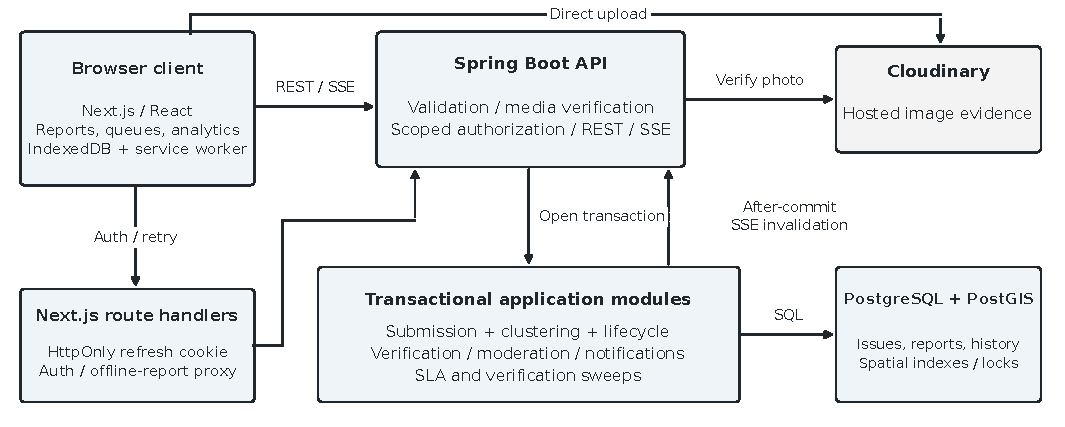
\includegraphics[width=\textwidth]{architecture.pdf}
\caption{Implemented component architecture and module interactions. Photo upload and evidence retrieval precede the transaction holding spatial locks. Database notifications commit with state changes; dashboard invalidations are emitted after commit.}
\label{fig:architecture}
\end{figure*}

A report contains a category, coordinates, declared GPS accuracy, description, device identifier, and hosted photo URL. A signed-in reporter identity is obtained from the validated token, not accepted from a client-supplied user identifier. The browser compresses and uploads the image to Cloudinary. In the normal media-verification configuration, the API validates the image origin, retrieves a deterministic rendition, and derives an authoritative perceptual hash before opening the report transaction. The demo configuration explicitly permits placeholder evidence and must be distinguished from that normal path.

The submission service checks durable quotas and optional idempotency records before invoking clustering. After commit, the API attaches display labels and returns a persistent issue reference. A citizen can subsequently track the ticket, eligible reporters can verify a repair, and scoped municipal users can act through the lifecycle. Supervisor corrections move reports between issues while retaining their original association evidence.

\subsection{Bounded Online Association}
Let report $r$ have longitude--latitude vector $x_r$, declared accuracy $a_r$ in metres, and category $k$. The implementation rejects accuracy above 150 m and uses an accuracy floor of 3 m. For members $i$ of an issue, it maintains
\begin{equation}
 \begin{aligned}
 w_i&=\frac{1}{\max(a_i,3)^2},\\
 W&=\sum_i w_i,\qquad S=\sum_i w_i x_i.
 \end{aligned}
 \label{eq:weights}
\end{equation}
The representative is $\mu=S/W$, with uncertainty proxy $\sigma=W^{-1/2}$. Updating $(W,S)$ requires constant arithmetic work. Longitude--latitude averaging is a local representative approximation; all decision distances use PostGIS geography in metres. Inverse-square weighting is an engineering model: browser accuracy values and correlated observations have not been calibrated as independent statistical standard deviations. Thus $\sigma$ is not presented as a validated confidence interval.

For category base radius $R_k$, the adaptive radius is
\begin{equation}
 R_{\mathrm{eff}}=R_k+\tfrac{1}{2}\min(a_r,60)+\tfrac{1}{2}\sigma.
 \label{eq:radius}
\end{equation}
Candidates must share the report's category and containing ward and be active, or recently resolved within the category's recurrence window. An indexed \texttt{ST\_DWithin} query uses search radius $1.5R_k+120$ m and returns at most five nearest issue identifiers. Geography distance and the index-assisted predicate follow PostGIS semantics~\cite{postgis}. After acquiring locks and rereading these candidates, the implementation evaluates the nearest one; it does not exhaustively search all alternatives after a refusal.

For representative distance $d$, three bands apply. If $d\leq R_{\mathrm{eff}}$, a merge is considered. If $R_{\mathrm{eff}}<d\leq1.5R_{\mathrm{eff}}$, the category selects either a flagged merge or a flagged separate issue. Beyond that band, a new issue is created. Safety-sensitive open-manhole reports use the separate-issue policy in the uncertain band. These bands are configurable rules rather than learned probabilities.

Before an otherwise admissible merge, the service projects the new representative $\mu'$. Let $B$ bound the maximum distance of existing members from $\mu$, and let $D$ be geodesic distance. The updated bound is
\begin{equation}
 B'=\max\{B+D(\mu,\mu'),\ D(x_r,\mu')\}.
 \label{eq:bound}
\end{equation}
The merge is permitted only if $B'\leq m_kR_k$, where $m_k$ is a category-specific extent multiplier. For every existing member $i$, the triangle inequality gives $D(x_i,\mu')\leq D(x_i,\mu)+D(\mu,\mu')\leq B+D(\mu,\mu')$. Together with the new member term in~\eqref{eq:bound}, this preserves the bound inductively from a singleton with $B=0$. An accepted ingest merge therefore bounds every pairwise member distance by $2m_kR_k$, provided the prior bound is valid. This is a geometric guarantee, not proof that the members describe one physical defect. Successive representative movements can inflate $B$ beyond the exact extent and cause unnecessary splits. A refused merge creates a flagged issue and retains the projected bound in its decision record.

Only representative and bound arithmetic is constant-time; candidate queries, lock waits, inserts, and distinct-reporter counting still contribute to ingest cost.

\subsection{Transactional Concurrency and Traceability}
The category and snapped coordinate cell, with grid spacing $0.002^\circ$, define a transaction-scoped advisory lock. This serializes submissions with the same lock key, including when no issue yet exists. Row locks then protect candidate representatives. PostgreSQL supports both advisory locks and transaction-scoped row locking~\cite{pglocks}. Because ordering and row-lock acquisition may observe different concurrent states, distances and running sums are reread after lock acquisition, consistent with PostgreSQL's documented locking caveats~\cite{pgselect}.

This strategy has a defined limitation. Adjacent cells acquire different advisory keys. If both initially contain no matching issue, reports straddling a boundary can concurrently create duplicates. Existing-row locks and post-lock rereads do not eliminate this empty-candidate race. The retained concurrency experiment tests identical locations, not exhaustive boundary configurations. Neighbourhood locking or another shared creation guard is a future extension.

Each report stores the decision type, representative distance, effective radius, and projected extent where applicable. These records explain why grouping occurred. Supervisor split/merge operations recompute geometry from actual members, preserve report identifiers, record moderation actions, and retain a merged ticket's redirect to its surviving issue. Merge policy preserves the more severe escalation and does not extend a deadline merely because work items were combined.

\subsection{Verification and Deadline Policy}
The nine states are NEW, ACKNOWLEDGED, ASSIGNED, IN\_PROGRESS, PENDING\_VERIFICATION, REOPENED, RESOLVED, CLOSED, and REJECTED. Fig.~\ref{fig:workflow} shows the normal path and correction loops. A declarative transition policy checks allowed edges, actor roles, department/ward scope, assignee identity, and evidence requirements. Crew members submit a proof image and a note of at least 20 characters to request verification. They cannot transition directly to RESOLVED or CLOSED.

\begin{figure}[t]
\centering
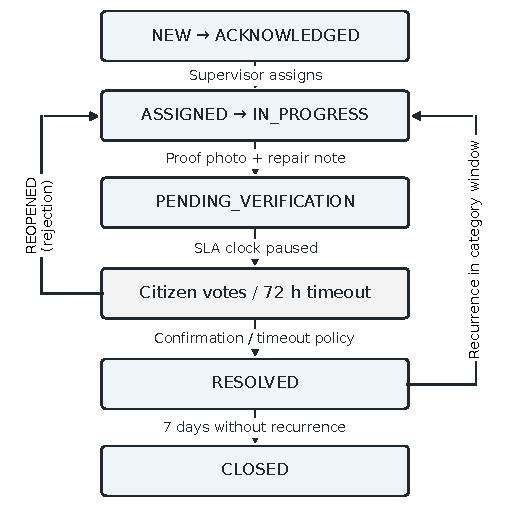
\includegraphics[width=\columnwidth]{workflow.pdf}
\caption{Primary issue workflow. SYSTEM settles citizen votes and timeouts. The rejection branch is available to supervisors/administrators from open states, including verification. Normal-profile time constants are shown.}
\label{fig:workflow}
\end{figure}

Only citizen accounts associated with a report on the issue may vote. The distinct-reporter count $n$ includes anonymous device identities, so it can exceed the number of eligible voters. The confirmation requirement is
\begin{equation}
 q=\min\{3,\max\{1,\lceil n/2\rceil\}\}.
 \label{eq:quorum}
\end{equation}
With confirmations $c$ and rejections $j$, settlement checks $j\geq1$ and $j\geq c$ first, reopening the issue if true. Otherwise it resolves when $c\geq q$, or after 72 h when $j=0$ or $c>j$. A timeout with $c=j=0$ is explicitly recorded as resolution without verification. Votes are unique per issue, verification round, and citizen; resubmitting a repair opens another round. Both vote-triggered and scheduled settlement hold the issue row lock and use the same tally rules.

This is a sequential settlement policy, not a vote of all reporters: one rejection before any confirmation reopens the issue immediately. Anonymous-only reports cannot produce eligible votes, and three confirmations can satisfy the capped quorum regardless of larger reporter counts. Resolution is therefore a workflow decision rather than independent evidence of physical repair quality; the no-response resolution rate makes one such evidence gap visible. After seven days in RESOLVED, SYSTEM, administrators, or supervisors may close the issue; staff remain excluded. Recurrence within the category's window reopens a resolved issue.

The service-level agreement (SLA) clock pauses during verification. Accumulated pause seconds are credited to the effective deadline, and scheduled workers handle breaches only while the clock runs. Escalation advances through department head, parent department head, ward officer, and administrator, with level four terminal but still publicly visible. Worker scheduling locks, row selection with \texttt{SKIP LOCKED}, unique escalation events, and compare-and-swap updates provide layered idempotency.

\section{System Design and Implementation}
\subsection{Persistent Evidence and APIs}
Fig.~\ref{fig:schema} summarizes the core relational model. Reports and issues are separate entities: multiple immutable observation identities can support one operational ticket. Issues store sufficient statistics, status, assignee, deadline fields, escalation, and verification round. Category rows supply base radii, extent multipliers, severity, recurrence windows, and SLA hours. Ward polygons constrain geographic ownership.

\begin{figure}[t]
\centering
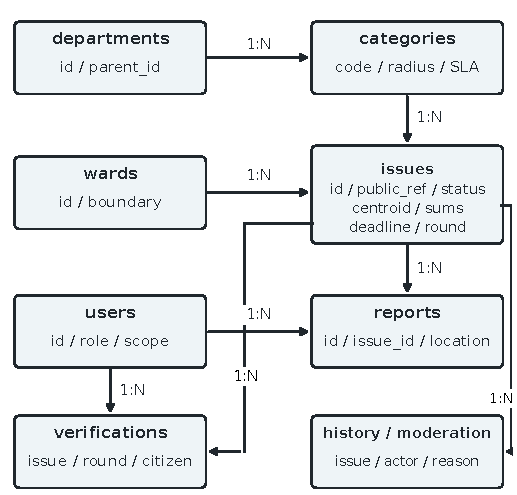
\includegraphics[width=\columnwidth]{schema.pdf}
\caption{Core database relationships. Lines point from referenced parent to dependent child and are labelled one-to-many. Reporter identity is nullable for anonymous reports. Auxiliary security, mail, and engagement tables are omitted.}
\label{fig:schema}
\end{figure}

Spatial columns use SRID 4326. The candidate index combines category with the geography cast of the representative through GiST and \texttt{btree\_gist}; ward boundaries and report locations also have spatial indexes. Partial indexes support overdue work and review queues. Foreign keys, round-specific uniqueness, and transaction boundaries complement service-level validation. Flyway migrations are treated as immutable once applied.

The versioned REST API separates public issue reads from scoped operational actions and audit views. Public responses omit private reporter fields and redacted descriptions. Ingest idempotency keys are scoped to an account or device and bound to a payload digest: identical retries return the stored result; changed payloads are refused.

\subsection{Priority and Accountability Analytics}
The implemented priority score is
\begin{equation}
 P=s_k+12\log_2(1+n)+0.15h+20e+15u,
 \label{eq:priority}
\end{equation}
where $s_k$ is configured category severity, $n$ is distinct reporter count, $h$ is elapsed age with accumulated pause credit removed, $e$ is escalation level, and $u$ is reopen count. Thresholds 25, 50, and 80 define medium, high, and critical bands. Anonymous reporter identities are device identifiers, which are weaker than verified person identities. Followers are excluded from $n$, so subscribing cannot buy urgency. The coefficients express project policy and have not been validated as an optimal municipal resource-allocation model.

Dashboard metrics expose backlog age, resolution time, deadline compliance, reopen rate, and resolution without verification. Compliance measures the repair claim against its deadline, separating municipal work time from citizen response time. Resolution-time samples below five completed issues are withheld. Server-sent events invalidate dashboard data after commit, with one-second coalescing.

\subsection{Security, Privacy, and Client Resilience}
Access tokens reside in browser memory and expire after 15 minutes. HttpOnly cookies hold rotating refresh tokens; persistent token families support reuse detection and revocation of future refreshes. Municipal roles require TOTP~\cite{totp} in the normal configuration, with encrypted secrets, replay counters, and single-use recovery codes. The demo profile bypasses mandatory enrolment.

Account/day quotas and nearby device-report checks use durable database state. Login token buckets remain process-local, so a multi-replica deployment needs a coordinated limiter. Image evidence checking, perceptual-hash reuse flags, suspicious-content screening, and reasoned public-description redaction support review; they are not validated fraud classifiers. Device rotation and coordinated accounts remain abuse limitations.

IndexedDB stores drafts and explicit offline submissions. Worker and foreground retries use idempotency keys without persisting bearer tokens; the submission route checks the original account. Background execution and installation remain unverified on physical devices.

Notifications are written in the state-change transaction; optional email uses a durable retrying outbox. Production email delivery and reviewed orphan-media cleanup remain operational follow-ups. CI, health checks, and encrypted backup/restore scripts support deployment but are not evidence of field reliability.

\section{Experimental Results and Discussion}
\subsection{Evidence and Experimental Protocol}
The evaluation addresses three questions: (RQ1) what association errors arise under the configured category policies; (RQ2) how the extent cap changes those errors on seeded and chain geometries; and (RQ3) what the retained concurrency and latency measurements establish within their tested scope. Citizen participation and physical repair outcomes are outside this evaluation.

The evidence comprises saved CSV assignments and summaries in \texttt{artifacts/evaluation}, Java integration experiments, and evaluation scripts. The accompanying source index maps claims to code and artifacts. The supplied \texttt{verify\_evidence.py} independently reconstructs pair counts for all 24 saved variants and records input hashes; all counts match the retained summaries. This verifies artifact consistency, not experimental repeatability: manuscript preparation did not rerun the service or benchmark workloads.

\textit{Quality.} The production-path experiment invokes the actual clustering service and PostGIS in an isolated Testcontainers database using the \texttt{postgis/postgis:17-3.4} image. A deterministic seed of 42 generates 250 observations in ten categories around Ludhiana, with reference time 2026-10-01. Reports are generated around labelled synthetic defects, with declared accuracies sampled between 5 and 50 m and Gaussian location perturbations scaled by accuracy. These labels describe the generator's intended defects; they are not field annotations. The baseline uses seeded category policies. Radius variants replay the retained observations in database timestamp/identifier order with a common base radius from 10 to 100 m in 5 m steps. This sweep also changes the extent threshold because that threshold is proportional to the base radius.

\textit{Ablation.} The seeded-corpus experiment compares configured extent multipliers with a nonbinding multiplier of 99.99, asserting that no cap refusal occurs in the latter variant. A second corpus places 18 ROAD\_DAMAGE observations 45 m apart along a line, with six intended defects of three reports each. It fixes the base radius at 60 m, uses a cap multiplier of 1.0 when enabled, and selects the flagged-merge uncertainty policy. This is a constructed stress test of a failure geometry; its parameters differ from the default road-damage multiplier of 2.5.

\textit{Concurrency.} A live HTTP script submits distinct-device reports at an identical coordinate in cohorts of 2, 5, 10, 20, and 50. It counts distinct returned issue identifiers. One cohort per size is retained, so these observations do not estimate a probabilistic race rate.

\textit{Latency.} The HTTP harness is configured for ten virtual users and 500 submissions at each of 1k, 10k, and 50k pre-existing spatially distributed issues. The retained aggregate CSVs contain no failures. A separate Java experiment performs 50 warmup ingests, resets the Micrometer timer, and records 300 direct-service ingests per scale. These measurements bypass the HTTP/controller path and are reported separately. The saved runs do not include a complete machine-resource and exact runtime manifest, independent replications, or per-request traces; tail quantiles cannot be independently reconstructed from the aggregates.

\subsection{RQ1: Quality and Error Distribution}
For each unordered pair of observations, a true positive (TP) shares both a ground-truth defect and a produced issue; a false positive (FP) shares only an issue; a false negative (FN) shares only a defect. Pairwise scores are
\begin{equation}
 \begin{aligned}
 \mathrm{Precision}&=\frac{\mathrm{TP}}{\mathrm{TP}+\mathrm{FP}},\quad
 \mathrm{Recall}=\frac{\mathrm{TP}}{\mathrm{TP}+\mathrm{FN}},\\
 F_1&=\frac{2\,\mathrm{Precision}\,\mathrm{Recall}}
 {\mathrm{Precision}+\mathrm{Recall}}.
 \end{aligned}
 \label{eq:metrics}
\end{equation}
The evaluator assigns precision or recall 1 when its denominator is zero. Consequently, categories with no positive pairs should not be interpreted as empirically perfect; the eight singleton stray-animal observations contribute no TP, FP, or FN pairs.

\begin{table}[t]
\caption{Baseline Pairwise Quality on 250 Synthetic Reports}
\label{tab:quality}
\centering\small
\begin{tabular}{@{}lrrrr@{}}
\toprule
Category & Reports & TP & FN & Recall\\
\midrule
Blocked drain & 21 & 16 & 0 & 1.000\\
Garbage accumulation & 27 & 32 & 0 & 1.000\\
Illegal dumping & 34 & 124 & 0 & 1.000\\
Open manhole & 48 & 93 & 112 & 0.454\\
Pothole & 18 & 13 & 0 & 1.000\\
Road damage & 41 & 174 & 0 & 1.000\\
Signage & 13 & 9 & 3 & 0.750\\
Streetlight & 26 & 70 & 29 & 0.707\\
Stray animal & 8 & 0 & 0 & ---\\
Water leak & 14 & 10 & 0 & 1.000\\
\midrule
All categories & 250 & 541 & 144 & 0.790\\
\bottomrule
\end{tabular}
\end{table}

The baseline yields 541 TP, zero FP, and 144 FN: precision 1.000, recall 0.790, and $F_1=0.883$. Table~\ref{tab:quality} shows that 112 of 144 missed pairs occur in OPEN\_MANHOLE. That category's tight radius, conservative extent policy, and uncertain-band separation are consistent with a preference against hiding distinct hazards, but the experiment does not isolate each mechanism's causal contribution. Open-manhole reports account for 19.2\% of observations but 77.8\% of missed pairs. Thus the aggregate score obscures a substantial category-specific splitting problem. Pairwise recall also weights a defect with $t$ reports by its $t(t-1)/2$ pairs, rather than giving every defect equal weight. Zero FP on this corpus does not guarantee zero erroneous merges in field data.

\subsection{RQ2: Extent-Cap and Radius Tradeoffs}
Table~\ref{tab:ablation} shows the principal result. On the seeded corpus, enabling the cap reduces recall from 0.872 to 0.790 and $F_1$ from 0.931 to 0.883. Both variants have zero FP. On the linear stress corpus, enabling the cap produces 18 TP, zero FP, and zero FN; the nonbinding variant yields 12 TP, 13 FP, and 6 FN. The cap removes the incorrect associations in this constructed chain case, but lowers seeded recall by 8.2 percentage points without reducing FP there. Its value therefore depends on the relative operational costs of combining different defects and splitting one defect across tickets. Those costs were not measured, so these results do not identify an optimal deployment policy.

\begin{table}[t]
\caption{Extent-Cap Ablation Through the Implemented Pipeline}
\label{tab:ablation}
\centering\small
\begin{tabular}{@{}llrrr@{}}
\toprule
Corpus & Extent cap & Precision & Recall & $F_1$\\
\midrule
Seeded & Enabled & 1.000 & 0.790 & 0.883\\
Seeded & Nonbinding & 1.000 & 0.872 & 0.931\\
Linear stress & Enabled & 1.000 & 1.000 & 1.000\\
Linear stress & Nonbinding & 0.480 & 0.667 & 0.558\\
\bottomrule
\end{tabular}
\end{table}

Fig.~\ref{fig:results} presents the common-radius sweep and direct-service latency. Aggregate $F_1$ rises from 0.383 at 10 m to 0.991 at 55 m and then plateaus through 100 m. Individual categories need not improve monotonically. As both the candidate radius and cap change, these results cannot isolate radius alone. The same corpus is used for this exploration, with no held-out deployment data; adopting 55 m everywhere would overinterpret a synthetic parameter sweep.

\begin{figure*}[t]
\centering
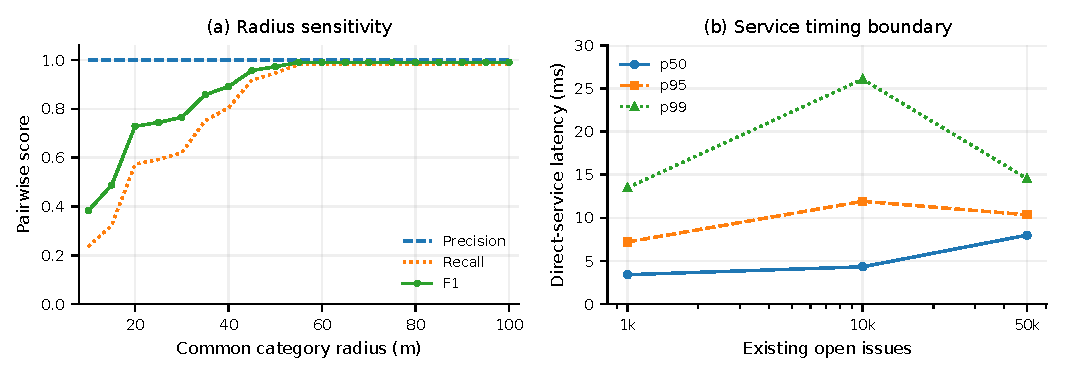
\includegraphics[width=\textwidth]{results.pdf}
\caption{Retained pipeline measurements. Left: aggregate pairwise scores under a common radius applied across categories, with the extent cap enabled. Right: direct-service Micrometer percentiles after 50 warmups and 300 measured ingests at each scale; these are distinct from the HTTP measurements in Table~\ref{tab:latency}. Lines connect measured configurations and do not imply unmeasured behavior.}
\label{fig:results}
\end{figure*}

\subsection{RQ3: Concurrency and Latency}
Each saved concurrency cohort returned one distinct issue identifier. Cohort elapsed times range from 545.4 to 939.8 ms; these are batch completion times, not per-request percentile estimates. The observation supports same-location serialization under the tested configuration while leaving the cell-boundary limitation unresolved.

\begin{table}[t]
\caption{Retained HTTP Ingest Latency: 500 Requests per Scale}
\label{tab:latency}
\centering\small
\begin{tabular}{@{}rrrrr@{}}
\toprule
Existing issues & p50 (ms) & p95 (ms) & p99 (ms) & Failures\\
\midrule
1,000 & 56.0 & 126.5 & 492.3 & 0\\
10,000 & 52.7 & 79.8 & 144.3 & 0\\
50,000 & 57.7 & 81.1 & 167.6 & 0\\
\bottomrule
\end{tabular}
\end{table}

Table~\ref{tab:latency} shows approximately stable HTTP medians, but its larger p99 at 1k precludes a monotonic scaling claim. Direct-service p50 values are 3.41, 4.33, and 8.00 ms; subtracting percentiles across these different workloads would not validly estimate overhead. Neither dataset characterizes production image downloads over an external network, limiting end-to-end generalization.

The repository audit records 275 backend passes, two skipped opt-in evaluations, and 82 frontend unit-test passes. PostGIS integration tests cover concurrency, lifecycle guards, verification, moderation, and escalation. These historical records provide implementation context; they are not a newly repeated audit, a field evaluation, or accessibility certification.

\subsection{Limitations and Threats to Validity}
\textit{External validity:} the corpus is small and synthetic, uses simplified ward geometries, and has no independently labelled real municipal incidents. Co-located defects, correlated GPS errors, moving targets, and cross-ward observations may behave differently. There is no municipality deployment study, user study, or measured improvement in repair time.

\textit{Internal and construct validity:} order-dependent assignment, nearest-candidate-only selection, strict ward containment, conservative bound accumulation, and the finite candidate search can change grouping. The radius sweep also varies extent limits, and replay tie ordering can differ from the seed's original stable chronological order. Pairwise scoring emphasizes larger defects and treats a geometric stress corpus according to deliberately constructed labels. Independent random-seed replications and comparative algorithm baselines are absent. Pair outcomes share observations and are not independent Bernoulli trials; confidence intervals would need to respect defect or dataset-level dependence. Verification policy is described and functionally tested, but participation, collusion resistance, and repair accuracy have not been empirically evaluated.

\textit{Concurrency and operation:} identical-coordinate tests do not prove global duplicate prevention. In-memory SSE fan-out and login limiters require additional coordination for multiple replicas. Photo retrieval, deployment cold starts, exact benchmark hardware, and long-running resource saturation are not characterized by the saved latency summaries. Production email, physical-device installation and assistive-technology checks, and reviewed media deletion remain operational follow-ups. The final audit's production verdict is conditional; implementation completeness is distinct from unrestricted production readiness.

\section{Conclusion and Future Scope}
NagrikSetu implements municipal work-item association and verification as one auditable workflow. Its bounded representative update retains constant arithmetic cost while category policies, geodesic checks, transaction boundaries, and correction tools constrain the consequences of uncertain observations. The citizen-verification loop separates a crew's repair claim from resolution and makes silent acceptance visible in public analytics.

Retained experiments show conservative grouping on 250 synthetic reports and an extent-cap tradeoff across ordinary and chain geometries. Same-location cohorts returned one issue, and saved local timings characterize short workloads with up to 50k existing issues; they do not establish sustained throughput. Field efficacy and comparative algorithm superiority remain untested.

Future evaluation should use independently labelled municipal incidents, multiple seeds, and comparative baselines under a common ticket-identity policy. Priority implementation work is uncertainty calibration, periodic exact-extent refresh, and neighbourhood locking across cell boundaries. Field studies must measure verification participation, abuse, accessibility, and repair outcomes before claims of municipal effectiveness are justified.

\bibliographystyle{IEEEtran}
\bibliography{references}
\end{document}
